%=============================================

%FIGURE: reference potentials

\begin{figure*}
\includegraphics[width=\textwidth]{figs/reference_potentials.eps}
\caption{Density distribution of the four reference galaxy potentials in Table \ref{tbl:referencepotentials}, for illustration purposes. These potentials are used throughout this work for mock data creation and potential recovery. [TO DO: Potential and/or population names in typewriter]}
\label{fig:ref_pots}
\end{figure*}

%=============================================

%====================================================================

%FIGURE: distribution of mock data in action and configuration space

\begin{figure*}
\plotone{figs/kks2WedgeEx_mockdata.eps}
\caption{Distribution of mock data in action space (2D iso-density contours, enclosing 80\% of the stars, the two central and the lower left panel) and configuration space (1D histograms, right panels), depending on shape and position of the survey observation volume and temperature of the stellar population. The parameters of the mock data model is given as Test \ref{test:kks2WedgeEx} in Table \ref{tbl:tests}. In the upper left panel we demonstrate the shape of the two different \texttt{wedge}-like observation volumes within which we were creating each a \texttt{hot} (red) and \texttt{cool} (blue) mock data set: a large volume centred on the Galactic plane (solid lines) and a smaller one above the plane (dashed lines). The distribution in action space visualizes how orbits with different actions also reach into different regions within the Galaxy. The 1D histograms on the right illustrate that qDFs generate realistic stellar distributions in galactocentric coordinates $(R,z,\phi,v_R,v_z,vT)$. \Wilma{[TO DO: fancybox Legend] [TO DO: Potential and/or population names in typewriter font]} \Jo{[TO DO: Jo suggests to make two or three separate figures out of this. I'm not yet convinced, as I think it is nice and tidy like this.]}} 
\label{fig:kks2WedgeEx}
\end{figure*}


%===========================================================================================================================================================================================

%====================================================================

%FIGURE: accuracy in the likelihood normalisation 

\begin{figure*}
\centering
\plotone{figs/normalisation_accuracy_4.eps}
\caption{Relative error  $\delta M_\text{tot}$ of the likelihood normalization $M_\text{tot}$ in Equation \ref{eq:relerrlikelihood} depending on the accuracy of the grid-based density calculation in Equation \ref{eq:tracerdensity} (and surrounding text). We show how $\delta M_\text{tot}$ varies with the spatial resolution (first column), velocity resolution (second column) and velocity integration range (third column) for two different potentials (\texttt{KKS-Pot} in the first row and \texttt{MW13-Pot} in the second row) and five different spherical observation volumes with radius $r_\text{max}$ (color coded according to the legend). (Test \ref{test:norm_accuracy} in Table \ref{tbl:tests} summarizes all model parameters.) $N_x$ is the number of spatial grid points in $R \in R_\odot \text{kpc} \pm r_\text{max}$ and $|z| \in [0,r_\text{max}]$ on which the density is evaluated according to Equation \ref{eq:tracerdensity}. The spatial resolution in $z$ is therefore $r_\text{max}/N_x$ and $2r_\text{rmax}/N_x$ in $R$. This choice is reasonable because the density is symmetric in $z$ and varies less in $R$ than in $z$, because the tracer scale length of the disk is much larger than its scale height. At each $(R,z)$ of the grid a Gauss-Legendre integration of order $N_v$ is performed over an integration range of $\pm n_\sigma$ times the velocity dispersion in $v_R$ and $v_z$ and $[0,1.5v_\text{circ}(R_\odot)]$ in $v_T$. $n_\sigma/N_v$ is therefore a proxy for the velocity resolution of the grid. (We vary $N_x$, $N_v$ and $n_\sigma$ separately and keep the other two fixed at the values indicated above the columns.) To arrive at the approximation $M_\text{tot,approx}$ for $M_\text{tot}$ in Equation \ref{eq:normalisation}, we perform a 40th-order Gauss-Legendre integration in each $R$ and $z$ direction of the interpolated density over the observed volume. We calculate the ``true'' normalization with high accuracy as $M_\text{tot} \approx M_\text{tot,approx}(N_x=20,N_v=56,N_\sigma=7)$. The black dots indicate the accuracy used in our analyses: It is better than $0.002\%$. Only for the smallest volume in the \texttt{MW13-Pot} (yellow line) the error is only $\sim 0.005\%$. This could be due to the fact, that, while we have analytical formulas to calculate the actions for the Staeckel potential \texttt{KKS-Pot} exactly, we have to resort to an approximate action calculation for the MW-like potential \texttt{MW13-Pot} (see Section \ref{sec:potentials}). \Wilma{[TO DO: Write $|\delta M_\text{tot}|$ on y-axis] [TO DO: Remove MW13-Pot completely from this plot, caption and test table] [TO DO: Caption too long]}}
\end{figure*}


%====================================================================


%====================================================================

%FIGURE: Triangle plot, shape of likelihood, multi-variate Gaussian

\begin{figure*}
\centering
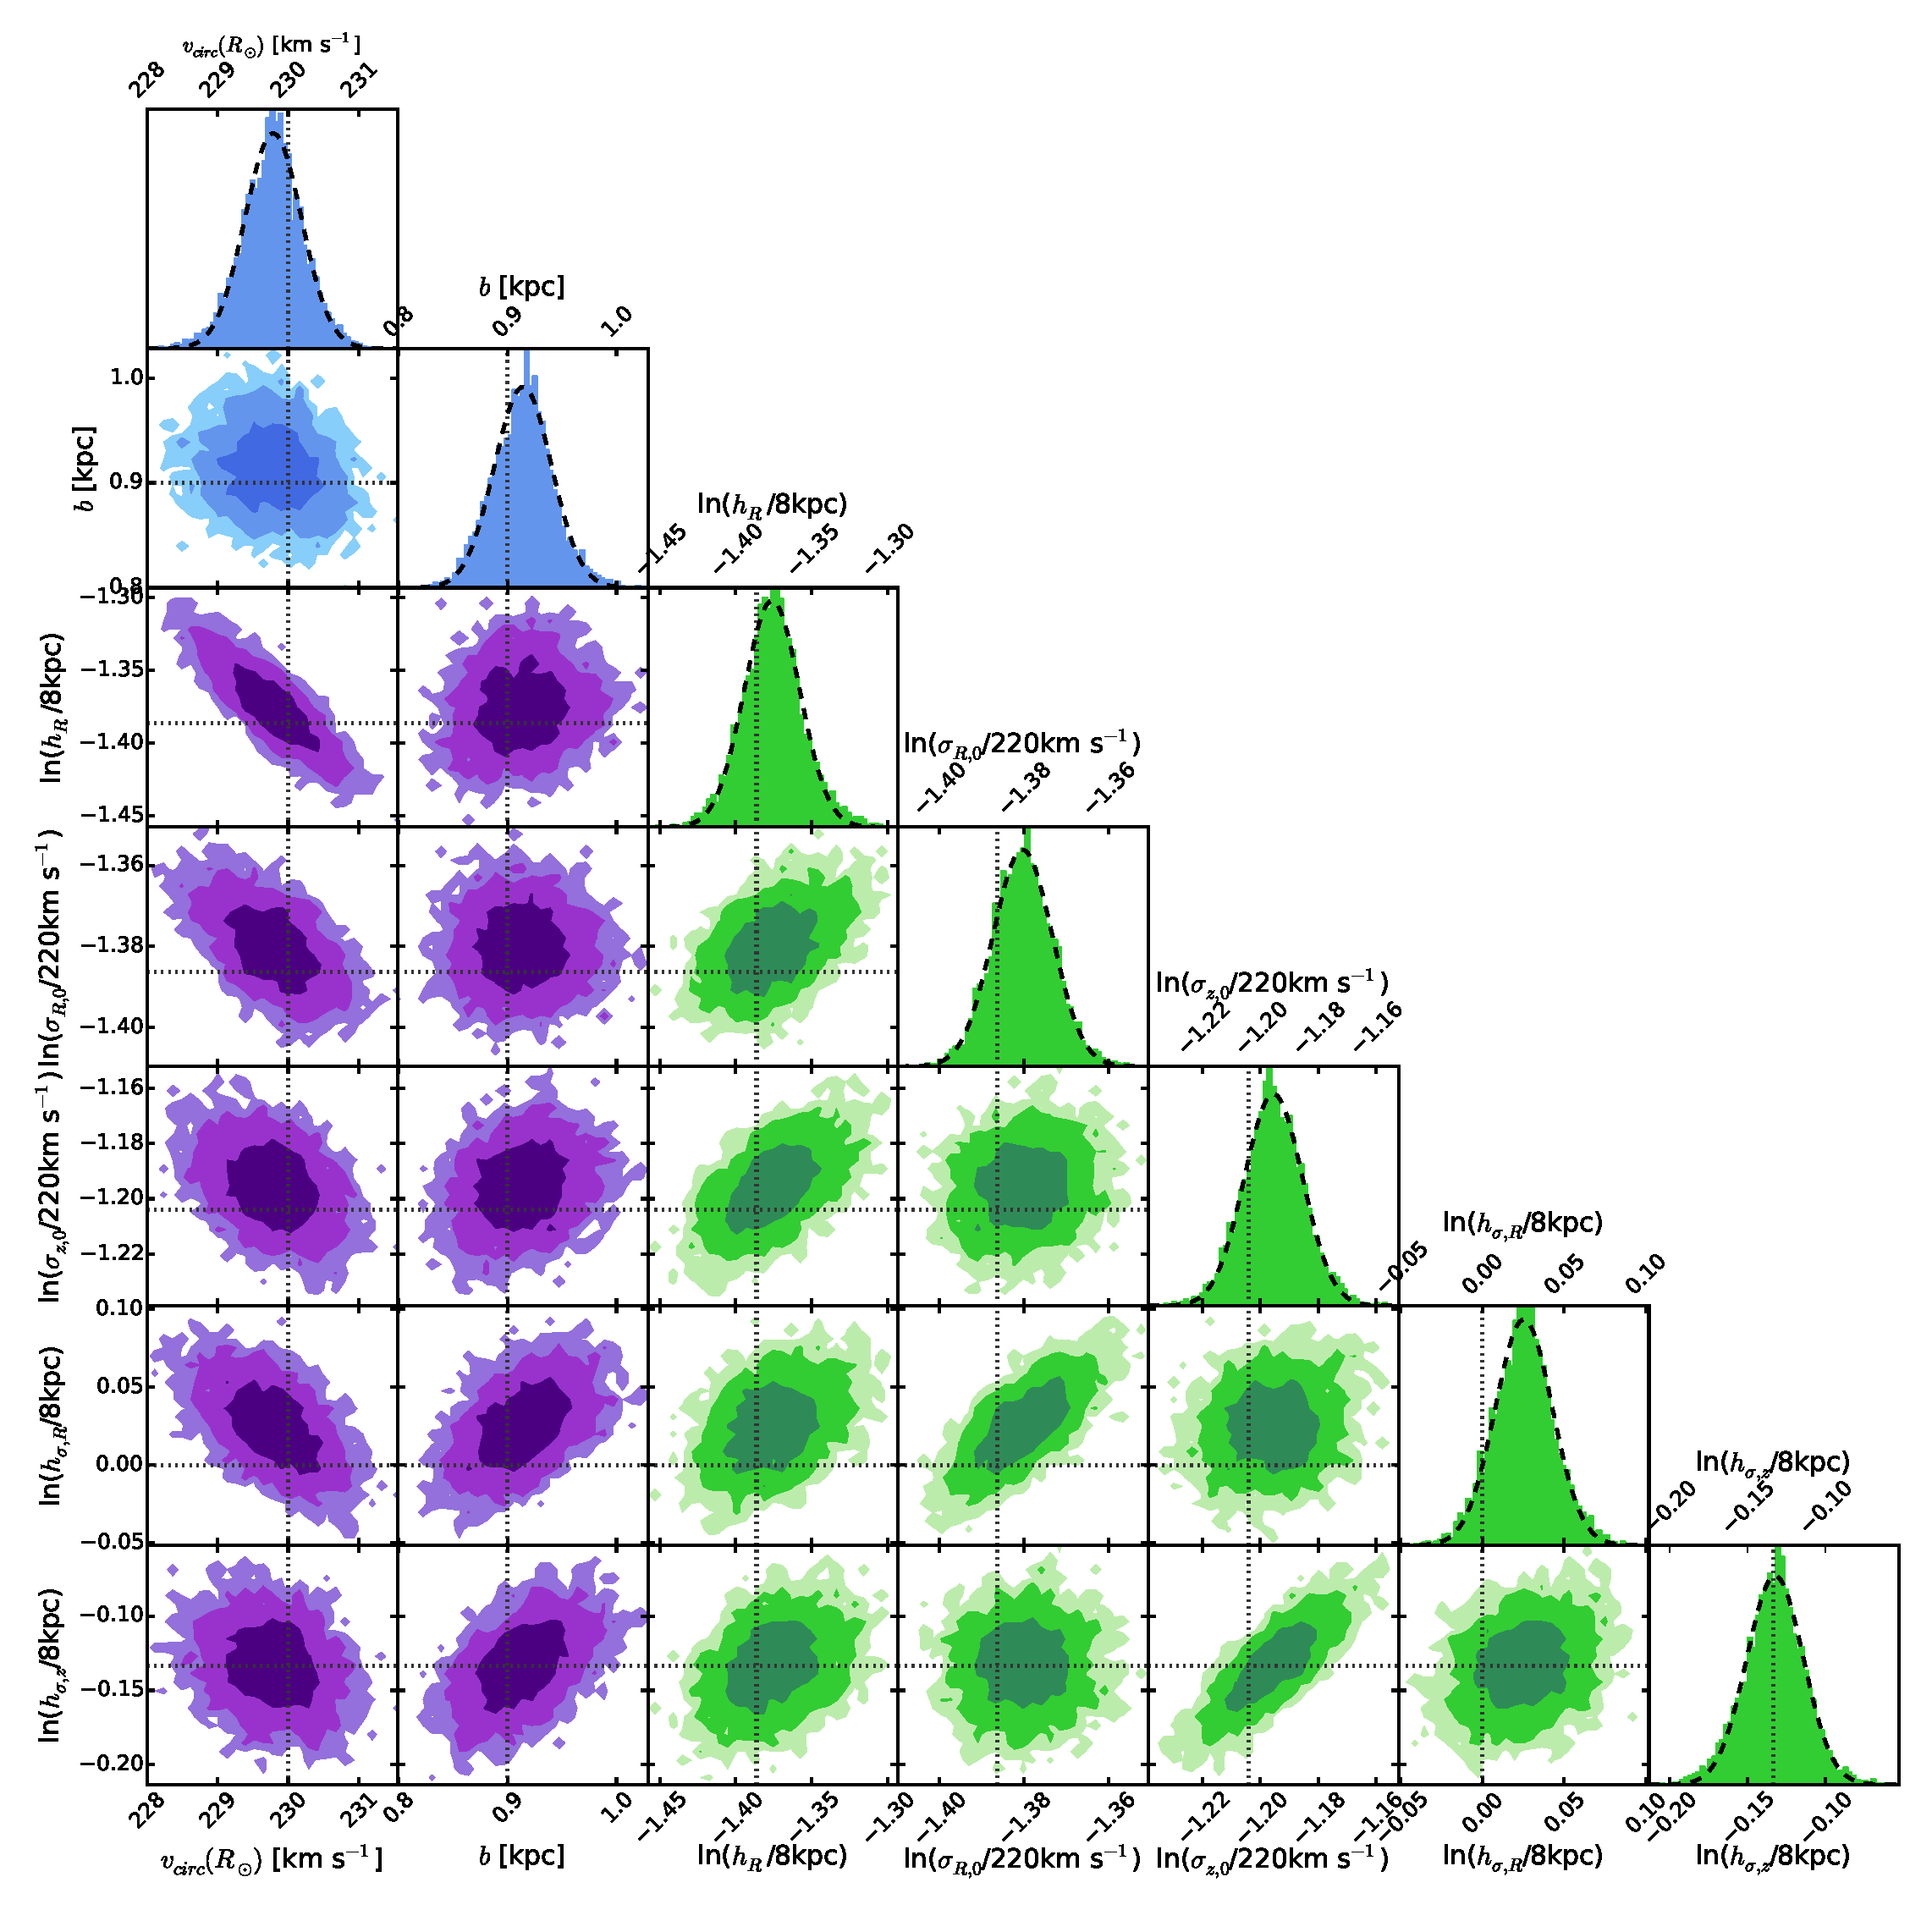
\includegraphics[width=0.7\textwidth]{figs/isoSphFlex_short_hot_2kpc_triangle_MCMC.eps}
%\plotone{figs/isoSphFlex_short_hot_2kpc_triangle_MCMC.eps}
\caption{The \pdf{} in the parameter space $\pmodel{} = \{p_\Phi,p_\text{DF}\}$ for one example mock data set created according to Test \ref{test:isoSphFlex} in Table \ref{tbl:tests}. Blue indicates the \pdf{} for the potential parameters, green the qDF parameters. The true parameters are marked by dotted lines. The dark, medium and bright contours in the 2D distributions represent 1, 2 and 3 sigma confidence regions \HW{[TO DO: HW: "likelihood vs. pdf - This is where this matters: is this a confidence on the data or on the parameters?" Don't understand, what he means...]}, respectively, and show weak or moderate covariances. This analysis was picked among five similar analyses, to have all 1 sigma contours encompass the input values \Jo{[TO DO: Jo didn't understand this sentence]}. The \pdf{} here was sampled using MCMC (with flat priors in $p_\Phi$ and  $\ln(p_\text{DF})$ to turn the likelihood in Equation \ref{eq:prob} into a full \pdf{}). Because only 10,000 MCMC samples were used to create the histograms shown, the 2D distribution has noisy contours. The dashed lines in the 1D distributions are Gaussian fits to the histogram of MCMC samples. This demonstrates very well that for such a large number of stars, the \pdf{} approaches the shape of a multi-variate Gaussian, as expected from the central limit theorem \Jo{[TO DO: Jo wrote, that he is not sure if the central limit theorem is directly relevant here]}. \Wilma{[TO DO: rename $h_{\sigma R}$ to $h_{\sigma,R}$, $\sigma_R$ to $\sigma_{R,0}$ and analogous for $z$]}}
\label{fig:isoSphFlex_triangleplot}
\end{figure*}

%====================================================================

%FIGURE: width of likelihood propto 1/sqrt(N)

\begin{figure}
\plotone{figs/sqrtNiso_Stddev_Vs_N.eps}
\caption{The width of the \pdf{} for two fit parameters found from analyses of 132 mock data sets vs. the number of stars in each data set. The mock data was created in the \texttt{Iso-Pot} potential and all model parameters are given as Test \ref{test:sqrtNiso} in Table \ref{tbl:tests}. The \pdf{} (using the likelihood in Equation \ref{eq:prob} \Wilma{[TO DO: CHECK]}) was evaluated and then a Gaussian was fitted to the marginalized \pdf{} of each free fit parameter. The standard error (SE) of these best fit Gaussians is shown for the potential parameter $b$ in kpc (red dots) and for the qDF parameter $\ln(h_R/8\text{kpc})$ in dimensionless units (blue). The black lines are fits of the functional form SE$(N_\text{sample}) \propto 1/\sqrt{N_\text{sample}}$ to the data points of both shown parameters. As can be seen, for large data samples the width of the \pdf{} behaves as expected and scales with $1/\sqrt{N_\text{sample}}$ as predicted by the central limit theorem. \Wilma{[TO DO: fancybox Legend] [TO DO: write pdf instead of likelihood on y-axis]}} 
\label{fig:sqrtNiso}
\end{figure}

%====================================================================


%FIGURE: central limit theorem is satisfied

\begin{figure}
\plotone{figs/isoSph_CLT_2.eps}
\caption{(Un-)bias of the parameter estimates: According to the central limit theorem the the best fit values for a large number of data sets, each containing a large number of stars, will follow the Normal distribution. To test this, we create 320 mock data sets, which come from two different stellar populations and five spherical observation volumes (see legends). All model parameters are summarized in Table \ref{tbl:tests} as Test \ref{test:isoSph_CLT}. Bias and relative standard error (SE) are derived from the marginalized \pdf{} for one potential parameter (isochrone scale length $b$ in first row) and one qDF parameter ($h_{\sigma,z}$ in second row). The second column displays a histogram of the 320 offsets. As it closely follows a Normal distribution, our modelling method is therefore well-behaved and unbiased. For the 32 analyses belonging to one model we also determine the mean offset and SE, which are overplotted in black in the first two columns (with $1/\sqrt{32}$ as error).  \HW{[TO DO: Is the scatter of the black symbols too large??? Is the reason for this numerical inaccuracies???]} \Wilma{[TO DO: Change test table accordingly, isochrone with b = 1.5 is not used anymore] [TO DO: Caption is too long. Make shorter.] [TO DO: $r_\text{max}$ instead of radius in legend] [TO DO: Leerzeichen fehlt in y-achsenbeschriftung]}}
\label{fig:isoSph_CLT}
\end{figure}

%====================================================================

%====================================================================

%FIGURE: Does shape and position of obs. volume matter?


\begin{figure*}[p]
\plotone{figs/wedFlexVol_bias_vs_SE.eps}
\caption{Bias vs. standard error in recovering the potential parameters for mock data stars drawn from four different test observation volumes within the Galaxy (illustrated in the upper right panel) and two different potentials (\texttt{Iso-Pot} and \texttt{MW13-Pot} from Table \ref{tbl:referencepotentials}). Standard error and offset were determined as in Figure \ref{fig:isoSph_CLT}. Per volume and potential we analyse four different mock data realisations; all model parameters are givenas Test \ref{test:wedFlexVol} in Table \ref{tbl:tests}. The colour-coding represents the different wedge-shaped observation volumes. The angular extent of each wedge-shaped observation volume was adapted such that all have the volume of $4.5 \text{ kpc}^3$, even though their extent in $(R,z)$ is different.  Overall there is no clear trend, that an observation volume around the sun, above the disk or at smaller Galactocentric radii should give remarkably better constraints on the potential than the other volumes. [TO DO: Write in Plot "... that all wedges have the same volume".]}
\label{fig:wedFlexVol_bias_vs_SE}
\end{figure*}


%====================================================================

%FIGURE: isoSphFlexIncompR in mock data space

\begin{figure}
\includegraphics[width=\columnwidth]{figs/isoSphFlexIncompR_mockdata.eps}
\caption{Selection function and mock data distribution for investigating radial incompleteness of the data. All model parameters are summarized as Test \ref{test:isoSphFlexIncomp}, Example 1, in Table \ref{tbl:tests}. The survey volume is a sphere around the sun and the percentage of observed stars is decreasing linearly with radius from the sun, as demonstrated in the left panel. How fast this detection/incompleteness rate drops is quantified by the factor $\epsilon_r$. Histograms for four data sets, drawn from two \MAPs{} (\texttt{hot} in red and \texttt{cool} in blue, see Table \ref{tbl:referenceMAPs}) and with two different $\epsilon_r$, 0 and 0.7, are shown in the right panel for illustration purposes. [TO DO: Potential and/or population names in typewriter font]} 
\label{fig:isoSphFlexIncompR_mockdata}
\end{figure}

%FIGURE: isoSphFlexIncompR

\begin{figure}
\centering
\plotone{figs/isoSphFlexIncompR_violins_2.eps}
\caption{Influence of wrong assumptions about the radial incompleteness of the data on the parameter recovery with \RM{}. Each mock data set was created having different incompleteness parameters $\epsilon_r$ (shown on the $x$-axis and illustrated in Figure \ref{fig:isoSphFlexIncompR_mockdata}) and the model parameters are given as Test \ref{test:isoSphFlexIncomp}, Example 1, in Table \ref{tbl:tests}. The analysis however didn't know about the incompleteness and assumed that all data sets had constant completeness within the survey volume ($\epsilon_r = 0$). The marginalized likelihoods from the fits are shown as violins. The green lines mark the true potential parameters (\texttt{Iso-Pot}) and the red and blue lines the true qDF parameters (\texttt{hot} \MAP in red and \texttt{cool} \MAP in blue), which we tried to recover. The \RM{} method seems to be very robust against small to intermediate deviations between the true and the assumed data incompleteness.} 
\label{fig:isoSphFlexIncompR_violins}
\end{figure}
